\begin{adjustwidth*}{}{-2.25in}
\textbf{{\large Exercises}}
\setlength{\columnsep}{25pt}
\begin{multicols*}{2}
\noindent Terms and Concepts \small
\begin{enumerate}[1)]
\item T/F: Implicit differentiation is often used when solving ``related rates'' type problems.
\end{enumerate} 

\noindent {\normalsize Problems} \small

\begin{enumerate}[1),resume]
\item Water flows onto a flat surface at a rate of $5$ cm$^3$/s forming a circular puddle $10$ mm deep. How fast is the radius growing when the radius is:
	\begin{enumerate}
	\item		$1$ cm?
	\item		$10$ cm?
	\item		$100$ cm?
	\end{enumerate}
	
\item A circular balloon is inflated with air flowing at a rate of $10$ cm$^3$/s. How fast is the radius of the balloon increasing when the radius is:
	\begin{enumerate}
	\item		$1$ cm?
	\item		$10$ cm?
	\item		$100$ cm?
	\end{enumerate}
	
\item Consider the traffic situation introduced in Example~\ref{Ex:3.1.Eg1}. How fast is the ``other car'' traveling if the officer and the other car are each $1/2$ mile from the intersection, the officer is traveling $50$ mph, and the radar reading is $70$ mph?

\item Consider the traffic situation introduced in Example \ref{Ex:3.1.Eg1}. How fast is the ``other car'' traveling if the officer and the other car are each $1$ mile from the intersection, the officer is traveling $60$ mph, and the radar reading is $80$ mph?

\item \label{exer:04_02_ex_07}An F-22 aircraft is flying at $500$ mph with an elevation of  $10,000$ ft on a straight--line path that will take it directly over an anti--aircraft gun. 

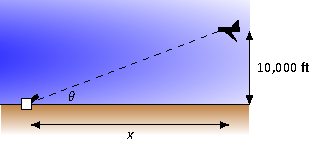
\includegraphics{figures/fig04_02_ex_07}

How fast must the gun be able to turn to accurately track the aircraft when the plane is:
\begin{enumerate}
\item	$1$ mile away?
\item	$1/5$ mile away?
\item	Directly overhead?
\end{enumerate}

\item An F-$22$ aircraft is flying at $500$ mph with an elevation of  $100$ ft on a straight--line path that will take it directly over an anti--aircraft gun as in Exercise \ref{exer:04_02_ex_07} (note the lower elevation here).

How fast must the gun be able to turn to accurately track the aircraft when the plane is:
\begin{enumerate}
\item	$1000$ feet away?
\item	$100$ feet away?
\item	Directly overhead?
\end{enumerate}

\item A $24$ ft. ladder is leaning against a house while the base is pulled away at a constant rate of $1$ ft/s.

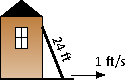
\includegraphics{figures/fig04_02_ex_09}

At what rate is the top of the ladder sliding down the side of the house when the base is:
\begin{enumerate}
\item	$1$ foot from the house?
\item	$10$ feet from the house?
\item	$23$ feet from the house?
\item	$24$ feet from the house?
\end{enumerate}

\item A boat is being pulled into a dock at a constant rate of $30$ ft/min by a winch located $10$ ft above the deck of the boat.

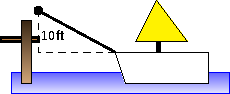
\includegraphics{figures/fig04_02_ex_10}

At what rate is the boat approaching the dock when the boat is:
\begin{enumerate}
\item	$50$ feet out?
\item	$15$ feet out?
\item	$1$ foot from the dock?
\item	What happens when the length of rope pulling in the boat is less than 10 feet long?
\end{enumerate}

\item An inverted cylindrical cone, $20$ ft deep and $10$ ft across at the top, is being filled with water at a rate of $10$ ft$^3$/min. At what rate is the water rising in the tank when the depth of the water is:
\begin{enumerate}
\item	1 foot?
\item	10 feet?
\item	19 feet?
\end{enumerate}
How long will the tank take to fill when starting at empty?

\item A hot air balloon lifts off from ground rising vertically. From $100$ feet away, a $5$' woman tracks the path of the balloon. When her sightline with the balloon makes a $45^\circ$ angle with the horizontal, she notes the angle is increasing at about $5^\circ$/min. 
\begin{enumerate}
\item		What is the elevation of the balloon?
\item		How fast is it rising?
\end{enumerate}



\end{enumerate}

%------------------------------------------
% END OF EXERCISES ON FIRST PAGE
%------------------------------------------
\end{multicols*}
\end{adjustwidth*}

\clearpage

\begin{adjustwidth*}{}{-2.25in}
\setlength{\columnsep}{25pt}
\begin{multicols*}{2}\small

\begin{enumerate}[1),start=12]

\item \label{exer:04_02_ex_12}A rope, attached to a weight, goes up through a pulley at the ceiling and back down to a worker. The man holds the rope at the same height as the connection point between rope and weight.

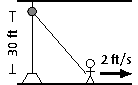
\includegraphics[scale=1.25]{figures/fig04_02_ex_12}

Suppose the man stands directly next to the weight (i.e., a total rope length of $60$ ft) and begins to walk away at a rate of $2$ ft/s. How fast is the weight rising when the man has walked:
\begin{enumerate}
\item	$10$ feet?
\item	$40$ feet?
\end{enumerate}
How far must the man walk to raise the weight all the way to the pulley?

\item Consider the situation described in Exercise \ref{exer:04_02_ex_12}. Suppose the man starts $40$ ft from the weight and begins to walk away at a rate of $2$ ft/s. 
\begin{enumerate}
\item	How long is the rope?
\item	How fast is the weight rising after the man has walked $10$ feet?
\item	How fast is the weight rising after the man has walked $40$ feet?
\item	How far must the man walk to raise the weight all the way to the pulley?
\end{enumerate}

\item A company that produces landscaping materials is dumping sand into a conical pile. The sand is being poured at a rate of $5$ ft$^3$/sec; the physical properties of the sand, in conjunction with gravity, ensure that the cone's height is roughly $2/3$ the length of the diameter of the circular base. 

How fast is the cone rising when it has a height of $30$ feet?

\item A baseball diamond is a square with sides $90$ feet long.  Suppose a baseball player is advancing from second to third base at the rate of $24$ feet per second, and an umpire is standing on home plate.  Let  $\theta$ be the angle between the third baseline and the line of sight from the umpire to the runner.  How fast is $\theta$ changing when the runner is $30$ feet from third base?
	
\item Sand is being dumped off a conveyor belt onto a pile in such a way that the pile forms in the shape of a cone whose radius is always equal to its height.  Assuming that the sand is being dumped at a rate of $10$ cubic feet per minute, how fast is the height of the pile changing when there are $1000$ cubic feet on the pile?
	
\item A swimming pool is $60$ feet long and $25$ feet wide. Its depth varies uniformly from $3$ feet at the shallow end to $15$ feet at the deep end, as shown below.
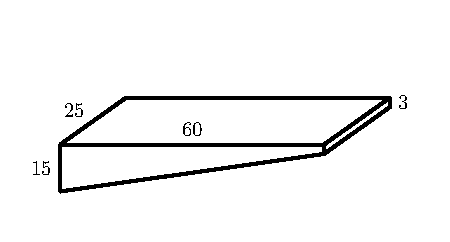
\includegraphics{figures/3_5_Ez3.eps}
Suppose the pool has been emptied and is now being filled with water at a rate of $800$ cubic feet per minute. At what rate is the depth of water (measured at the deepest point of the pool) increasing when it is $5$ feet deep at that end?  Over time, describe how the depth of the water will increase:  at an increasing rate, at a decreasing rate, or at a constant rate.  Explain.

\end{enumerate}

%---------------------------------------------
% END OF EXERCISES ON SECOND PAGE
%---------------------------------------------
\end{multicols*}
\end{adjustwidth*}

\afterexercises